%--------------------------------------
% Create title frame
\titleframe

%--------------------------------------
% Table of contents
\begin{frame}{Overview}
  \setbeamertemplate{section in toc}[sections numbered]
  \tableofcontents
\end{frame}

%--------------------------------------

\begin{frame}{Content of this lecture}
In this lecture we review microgrids architectures, that is which components form a microgrid and how to interconnect them.

\end{frame}

\section{AC Architectures}

\begin{frame}{AC grids}
An alternating current (AC) microgrid is a microgrid where components are coupled through one AC bus, or an AC network, potentially with two voltage levels if the network is long (e.g. a few kilometers).
\begin{itemize}
  \item Most microgrids are AC
  \item Typically, AC microgrids where the demand $>10 \mathrm{~kW}$ are three-phase!
  \begin{itemize}
    \item Required if you want to connect to the public grid (in Belgium)
    \item Equipment in general require less components per unit of power transferred
    \item Easy to generate a rotating field for motors
    \item (Three-phase power transfer is a constant expression, if the phases are balanced)
  \end{itemize}
\end{itemize}

\end{frame}

\begin{frame}{Grid topologies}
Most common: \textbf{radial} architecture

\begin{itemize}
  \item Subject to availability issues (one single path to a load)
\end{itemize}

Alternatives:
\begin{enumerate}
  \item provide a \textbf{redundant path} to each load (more robust than radial)
  \item provide \textbf{spatially diverse paths} (more robust than 1 )
  \item \textbf{ring-type} distribution (Can isolate a fault and still feed all but problematic zone)
  \item \textbf{ladder type} distribution (yet more connection possibilities)
\end{enumerate}

Note: a more complex system also needs more complex protection schemes.
\end{frame}

\begin{frame}{AC coupling example}

  \begin{columns}
  \begin{column}{0.4\textwidth}
    Let's take the example of a house or a small company that is running at low-voltage $(230 \mathrm{~V}$ or 400 V$)$ and has a grid connection 
    plus a backup diesel generator, some PV panels, a battery, and some appliances.\\
  \end{column}
  \begin{column}{0.55\textwidth}
    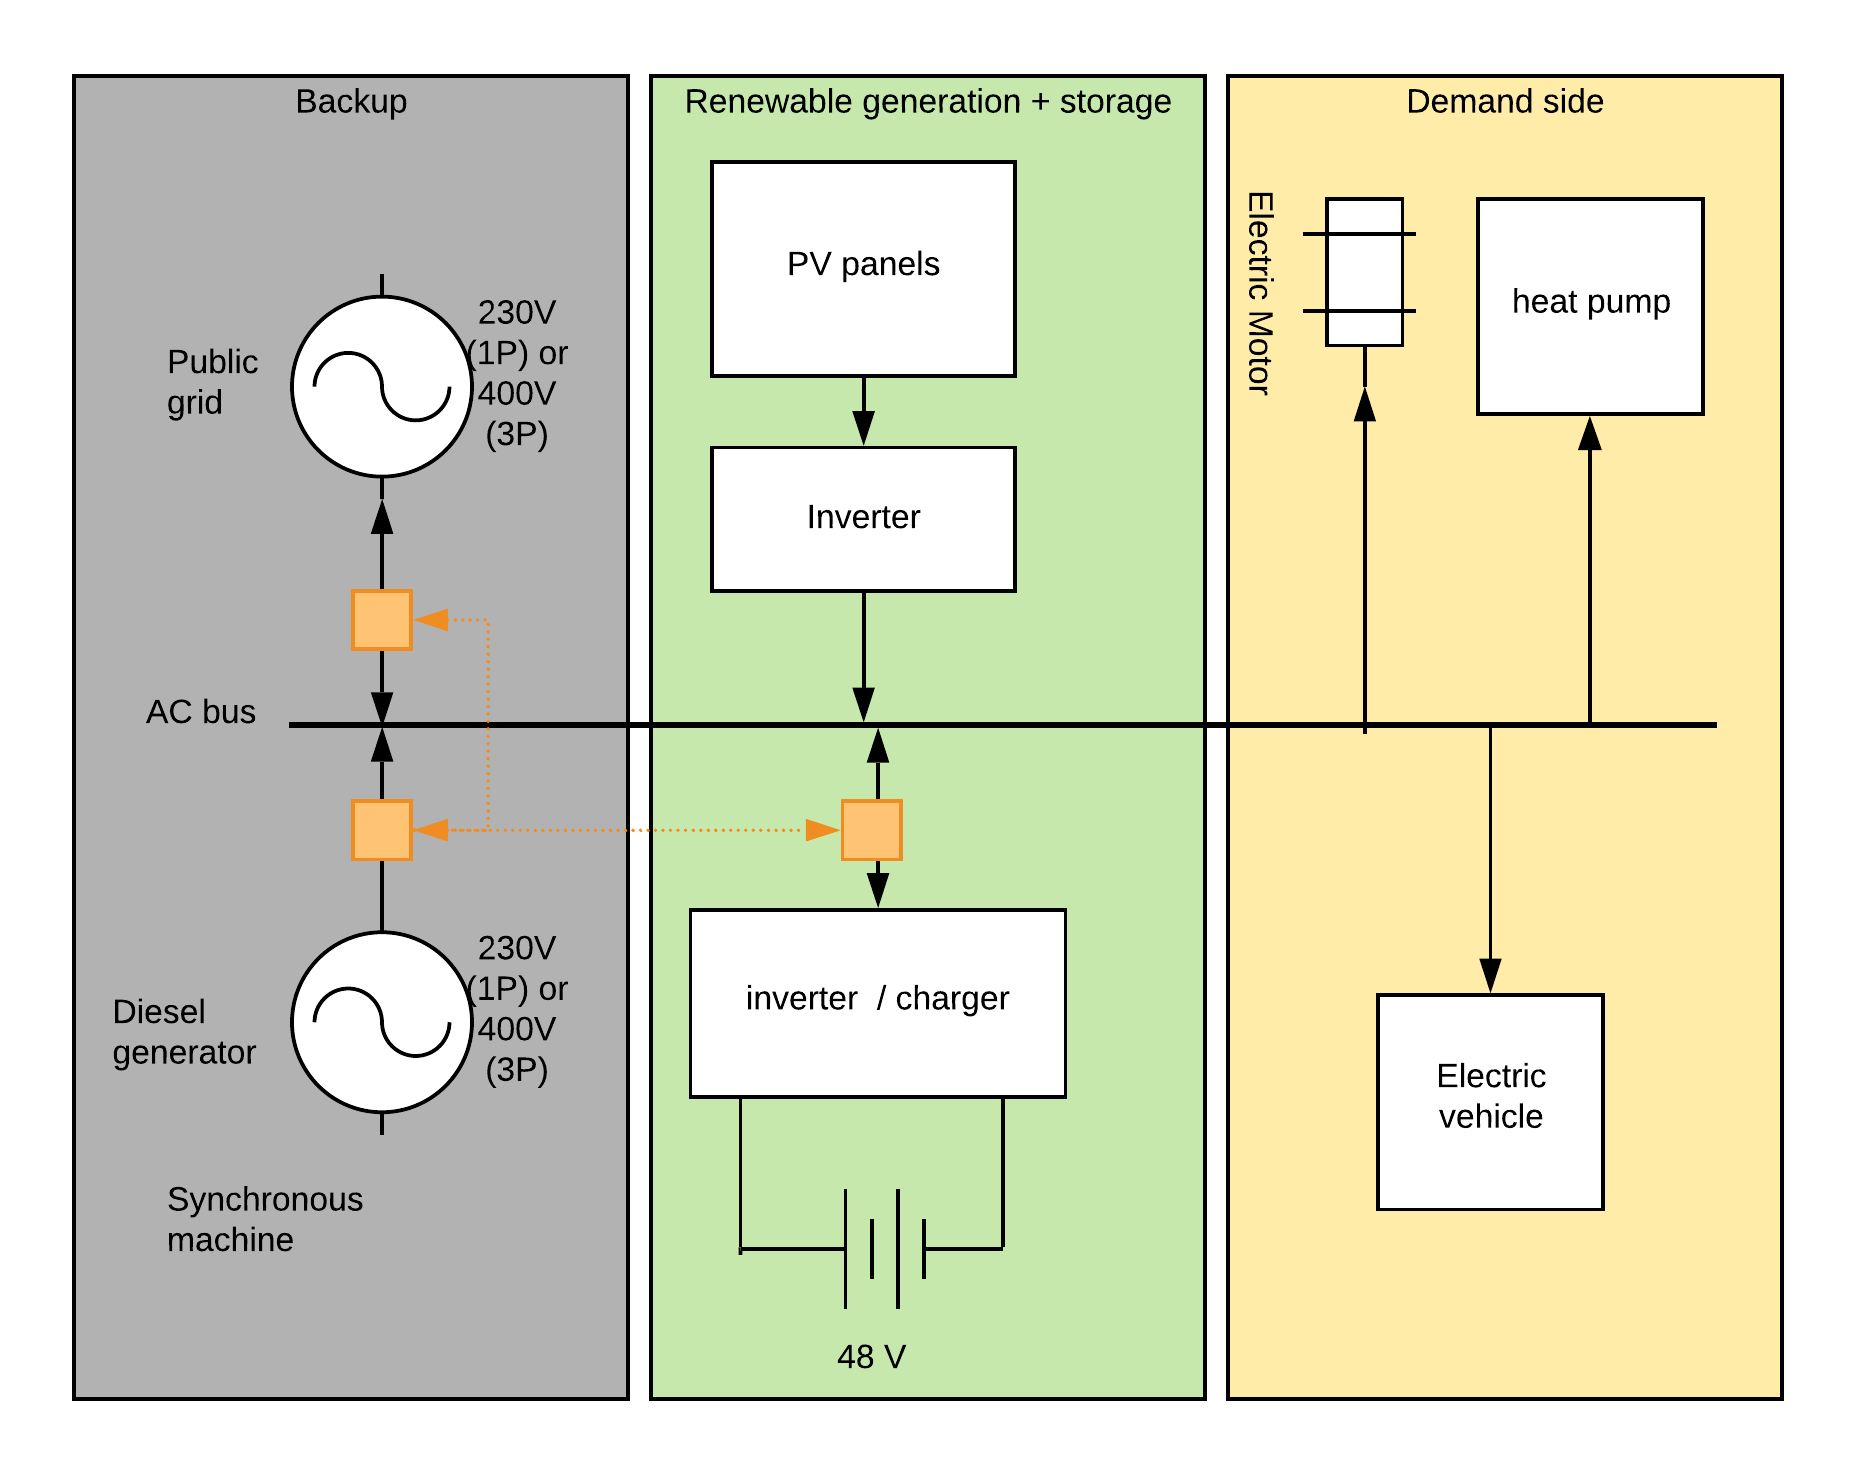
\includegraphics[width=\textwidth]{images/AC_coupling.png}
  \end{column}
\end{columns}

\end{frame}

\begin{frame}{Automatic transfer switches}
\begin{center}
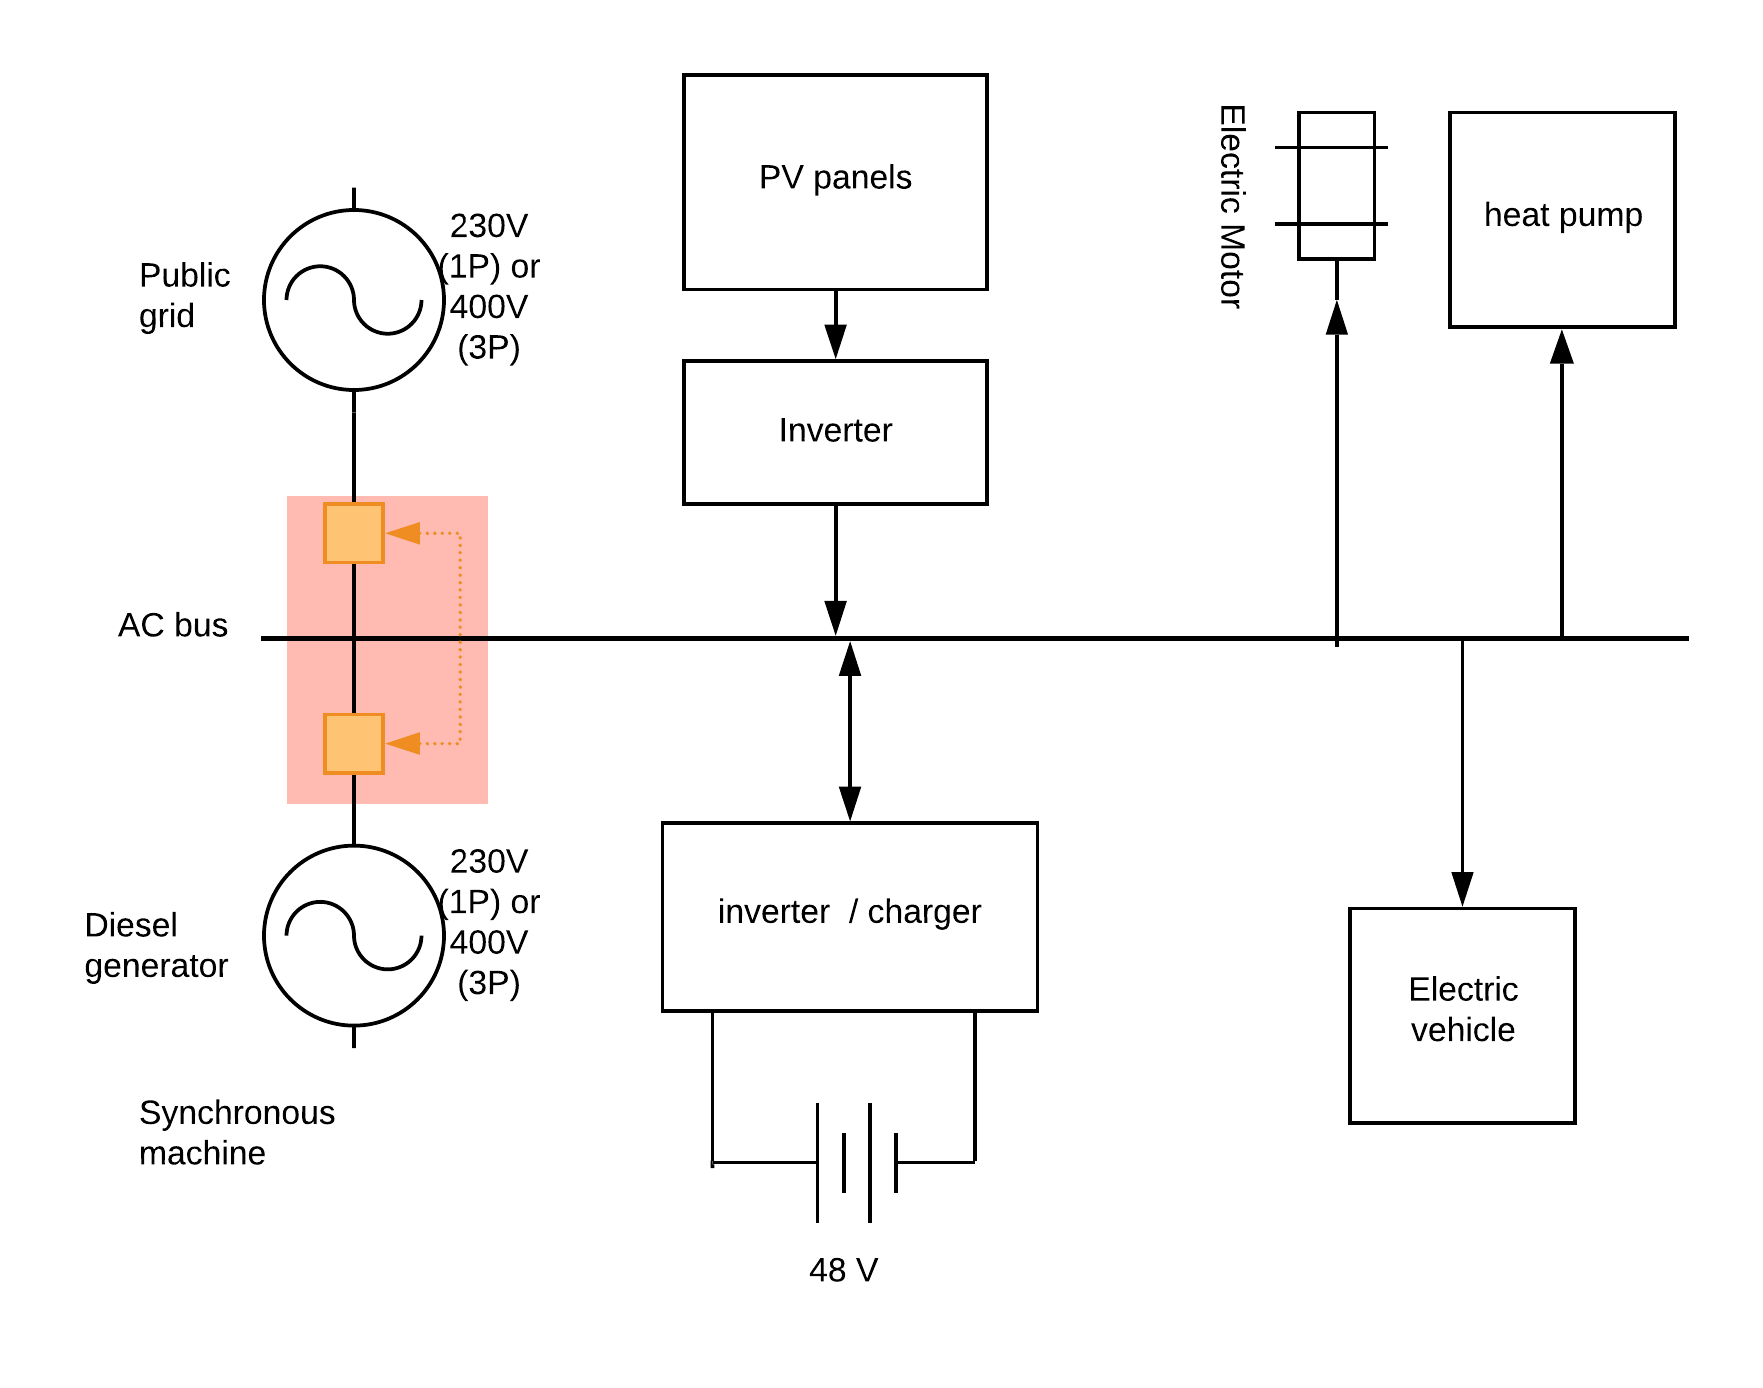
\includegraphics[width=0.65\textwidth]{images/AC_coupling_ATS.png}
\end{center}
\end{frame}

\begin{frame}{Automatic transfer switch principle}

  \centering
  \href{https://youtu.be/883JgMK9EGg}{
\includegraphics[width=0.65\textwidth]{images/video_ATS.png}}

\end{frame}

\begin{frame}[allowframebreaks]{Power electronics interfaces}
Power electronic circuits are interfaces
\begin{itemize}
  \item between devices (DERs and loads) and the power distribution grid
  \item between the microgrid and the distribution grid (PCC)
\end{itemize}

Purpose: enable a controllable (bidirectional) flow between devices\\

*DER: sources of electric power that are not directly connected to a bulk power transmission system. Distributed energy resources include both generators and energy storage technologies. (T.Ackermann, G.Andersson, and L.Söder, "Distributed Generation: A Definition," Electric Power Systems Research, vol. 57, issue 3 , April 2001, pp. 195-204.)

\end{frame}


\begin{frame}{Types of power electronics interfaces}

  
\begin{columns}
  \begin{column}{0.55\textwidth}
    \textbf{Grid-following converters} (Fig (b)): can be represented as an ideal current source setting the active and reactive power injected into / withdrawn from the grid.
    
    \textbf{Grid-forming converters} (Fig (a)): can be represented as an ideal AC voltage source setting the voltage amplitue and frequency of the local electrical grid.
    
    \textbf{Grid-supporting converters} (Fig (c)): "inbetween the two others", implementing functions to support the grid, e.g. droop control.\\
  \end{column}
  \begin{column}{0.4\textwidth}
    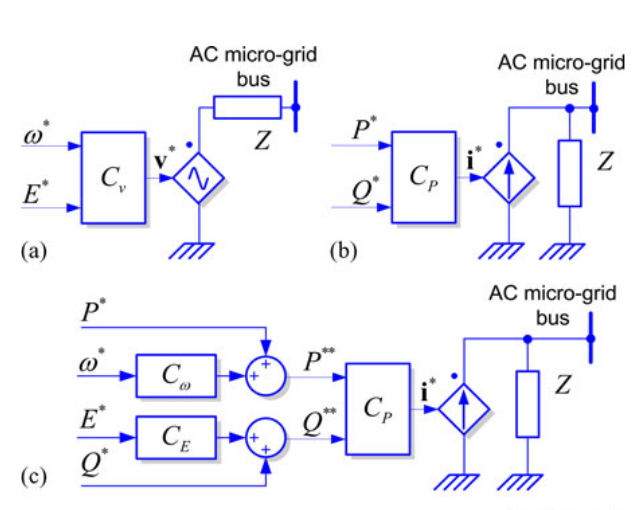
\includegraphics[width=\textwidth]{images/types_of_converters_2.png}
  \end{column}
\end{columns}
{\footnotesize From \textit{Rocabert, J., Luna, A., Blaabjerg, F., \& Rodríguez, P. (2012). Control of power converters in AC microgrids. IEEE Transactions on Power Electronics, 27(11), 4734-4749. \href{https://doi.org/10.1109/TPEL.2012.2199334}{https://doi.org/10.1109/TPEL.2012.2199334}}}

\end{frame}

\begin{frame}{Example: solar inverter}

  \begin{columns}
  \begin{column}{0.35\textwidth}
    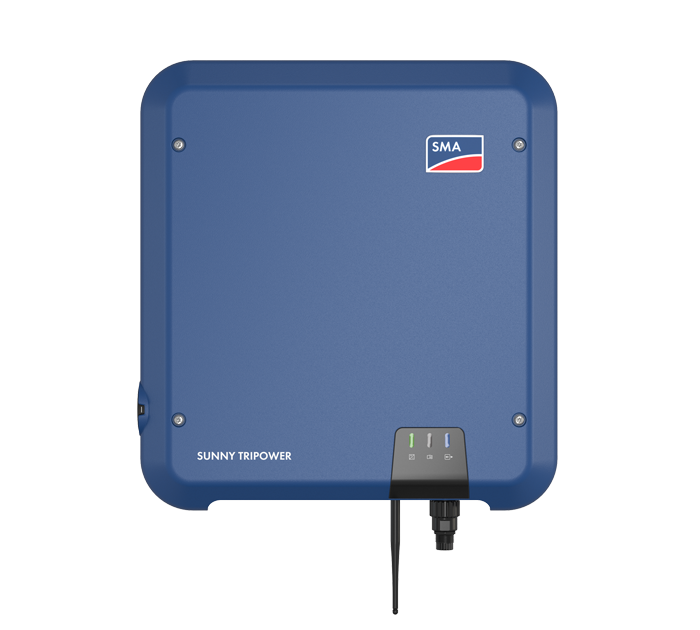
\includegraphics[width=\textwidth]{images/sma-sunny-tripower.png}\\
  
  \end{column}
  \begin{column}{0.5\textwidth}
    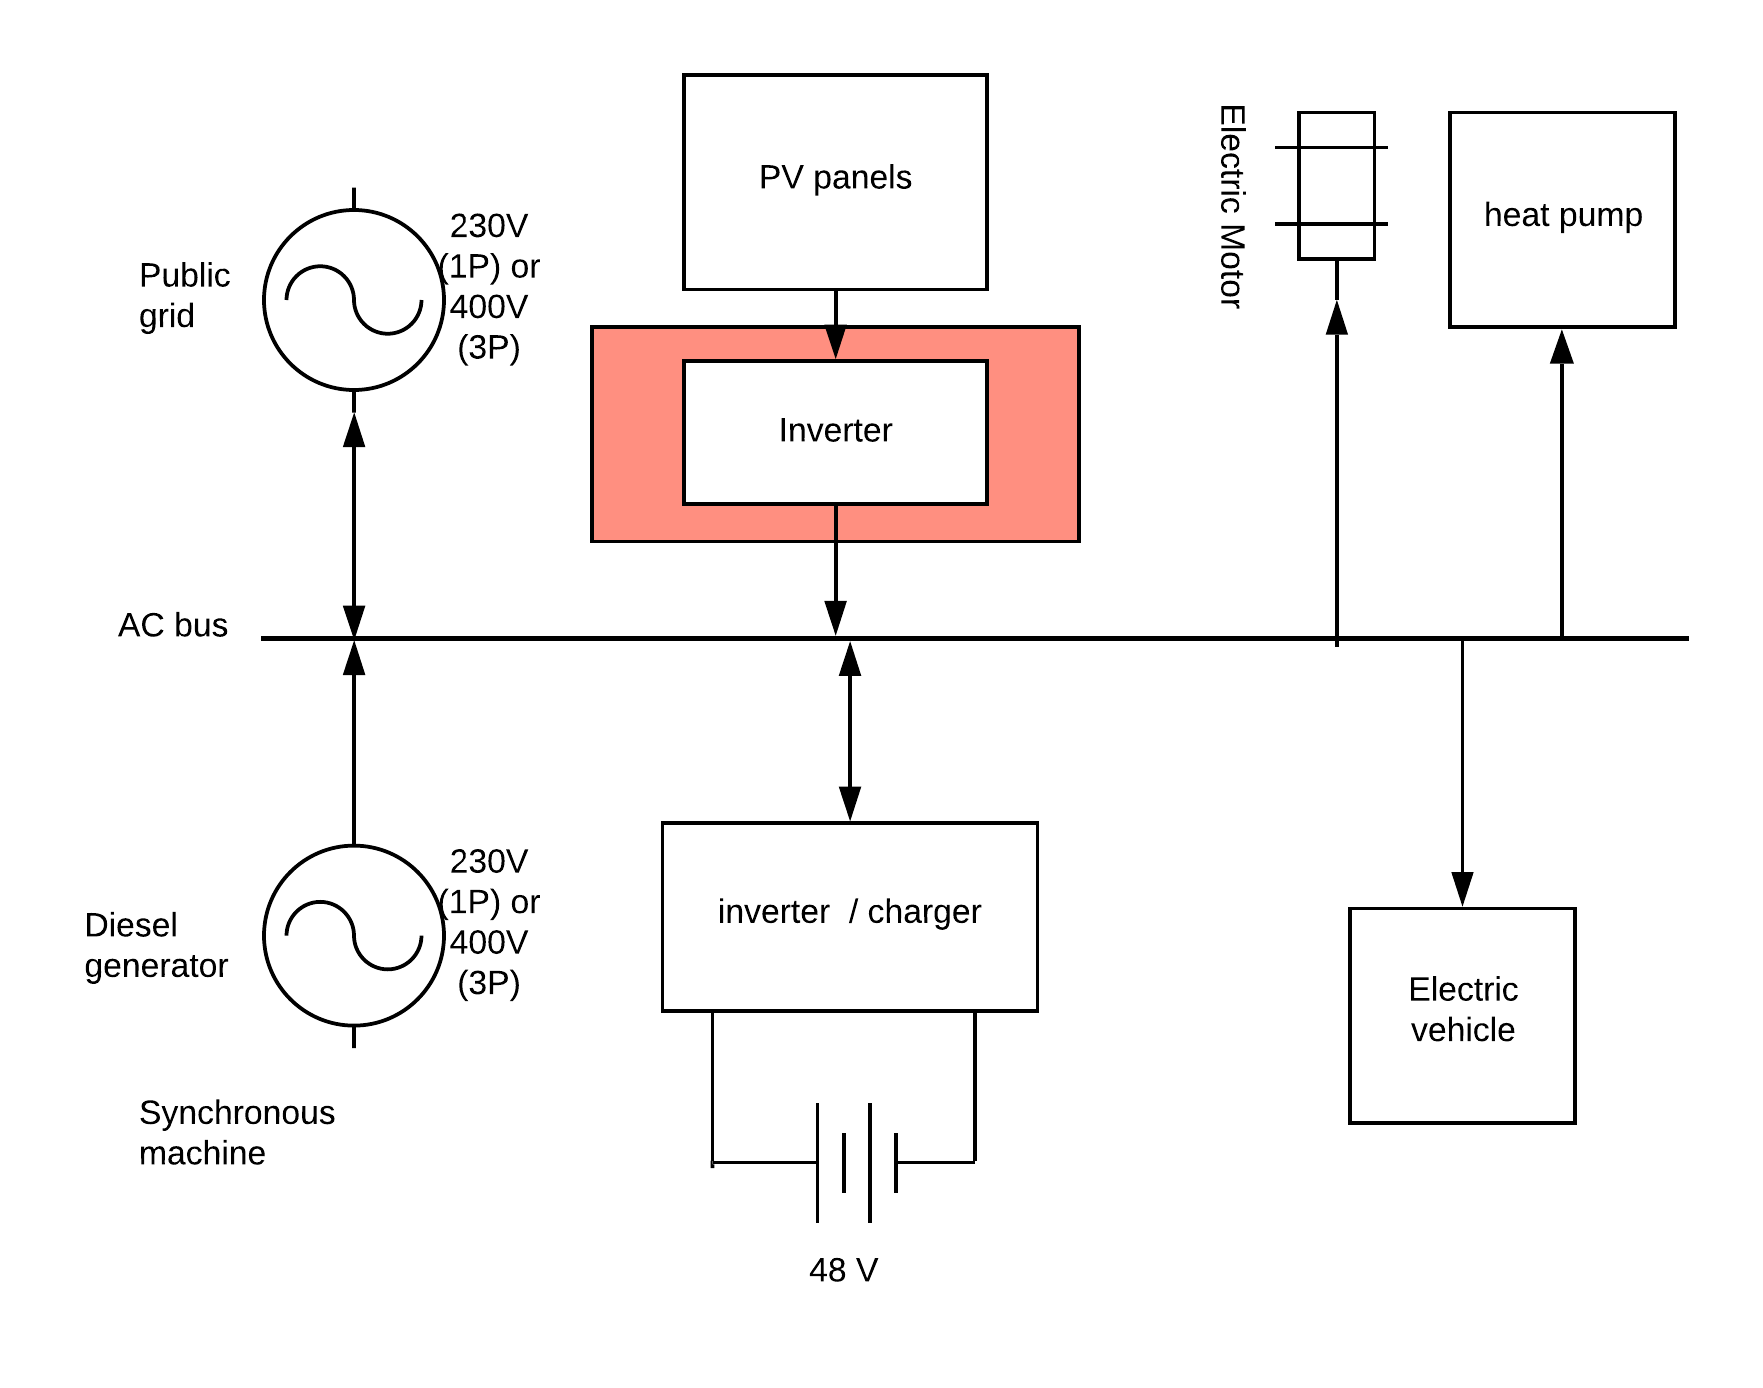
\includegraphics[width=\textwidth]{images/AC_coupling_inverter.png}

  \end{column}
\end{columns}

Here it is a three-phase inverter from SMA. Source: website of SMA

Requires a network signal to work! \textbf{Grid following}.
\end{frame}

\begin{frame}{Example: Vehicle to grid}
\begin{center}
  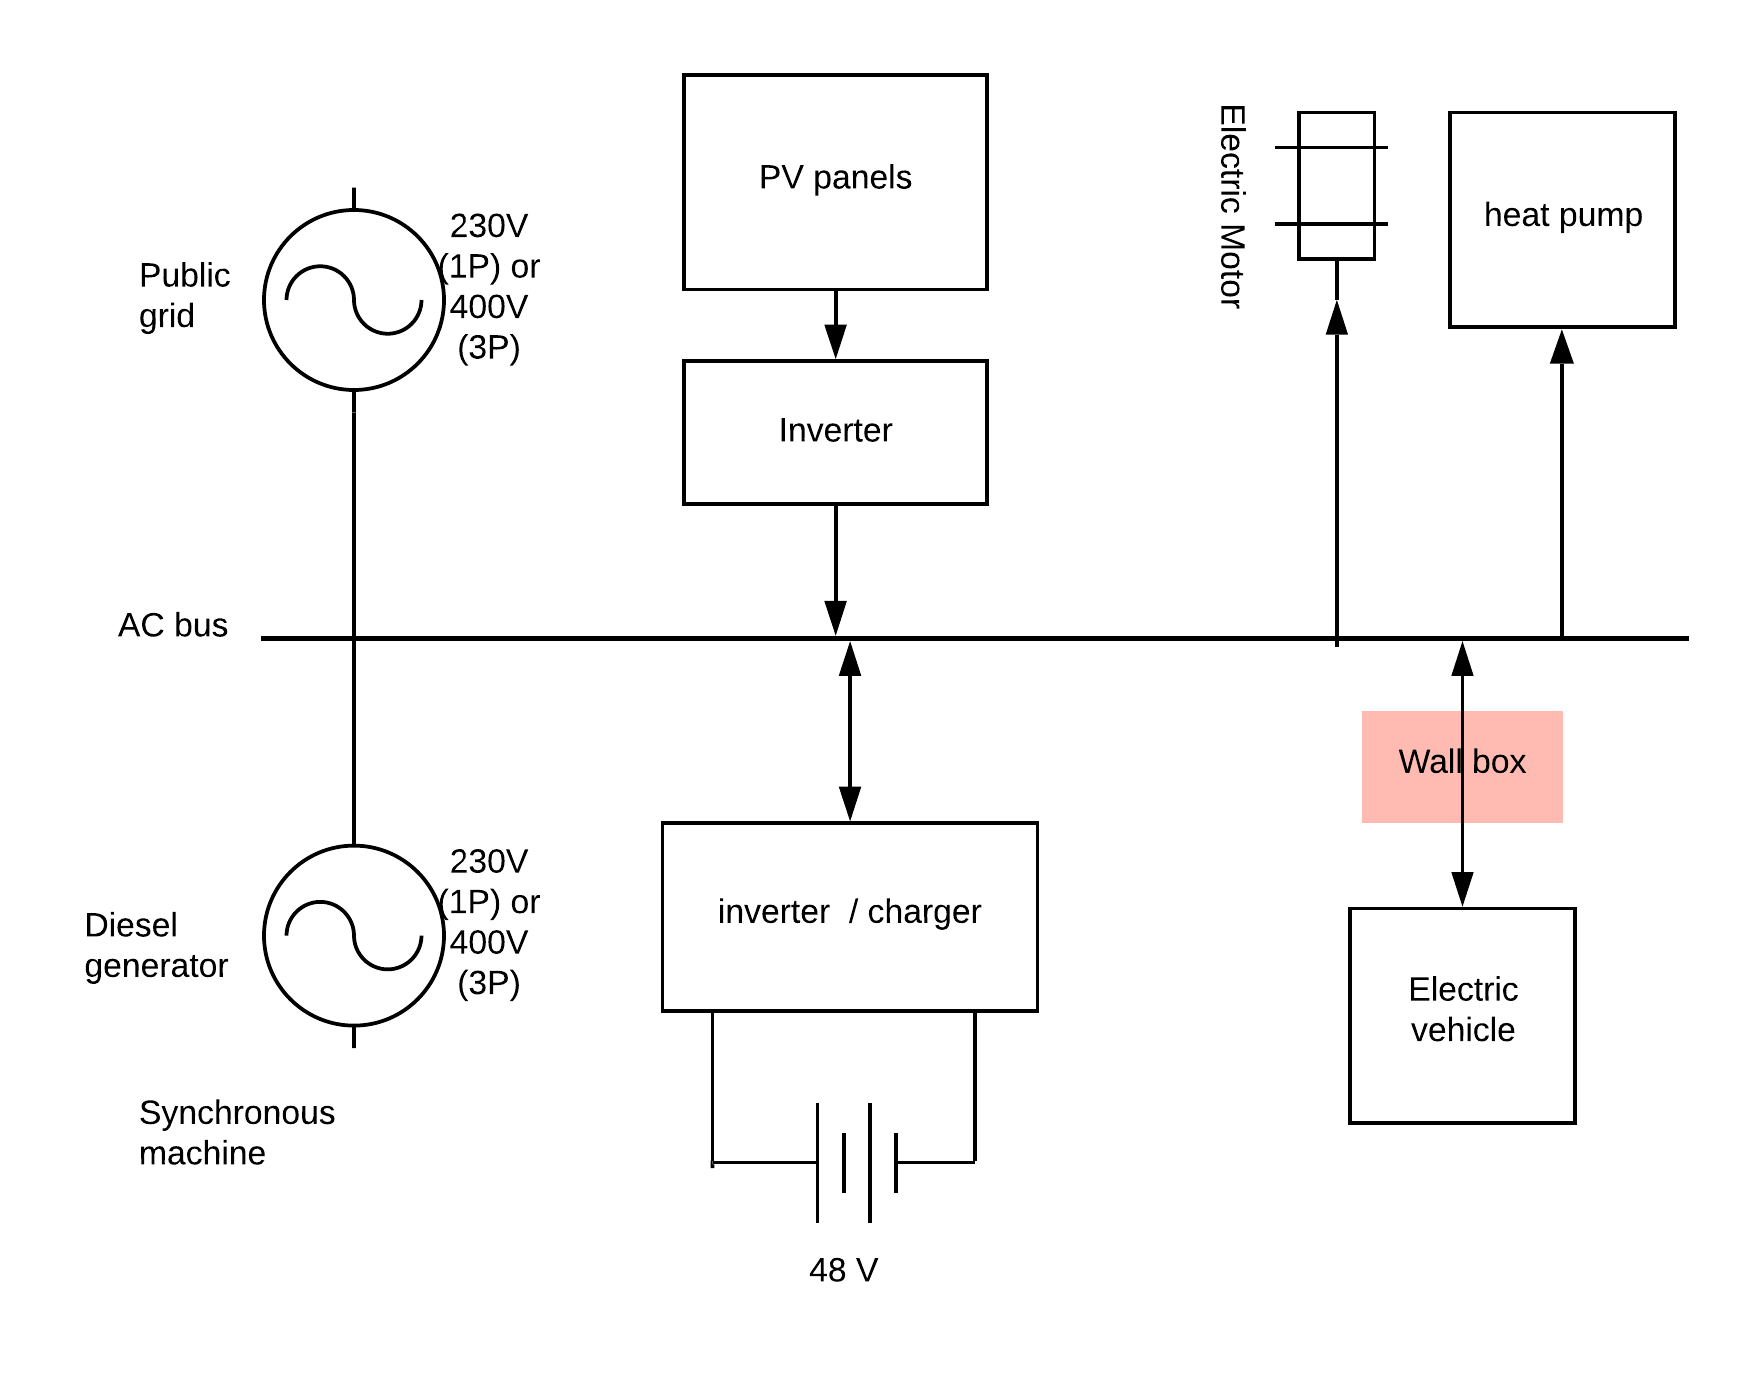
\includegraphics[width=0.6\textwidth]{images/AC_coupling_V2G.png}
\end{center}
\end{frame}

\begin{frame}{The car that does much more }
  \begin{center}
  \href{https://youtu.be/5FAsadUM26I}{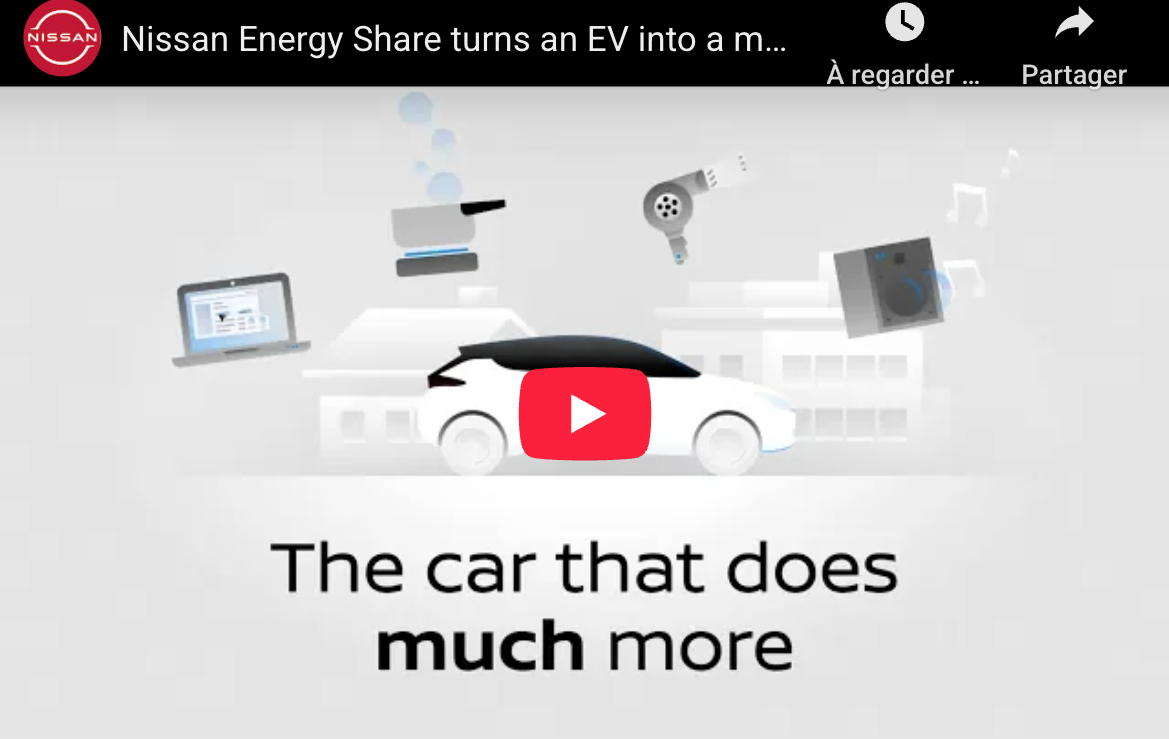
\includegraphics[width=0.5\textwidth]{images/video_NISSAN_V2G.png}}
  \end{center}
\end{frame}

\begin{frame}{Example: Automatic transfer switch, grid forming inverter \& battery charger}
  \begin{columns}
  \begin{column}{0.45\textwidth}
    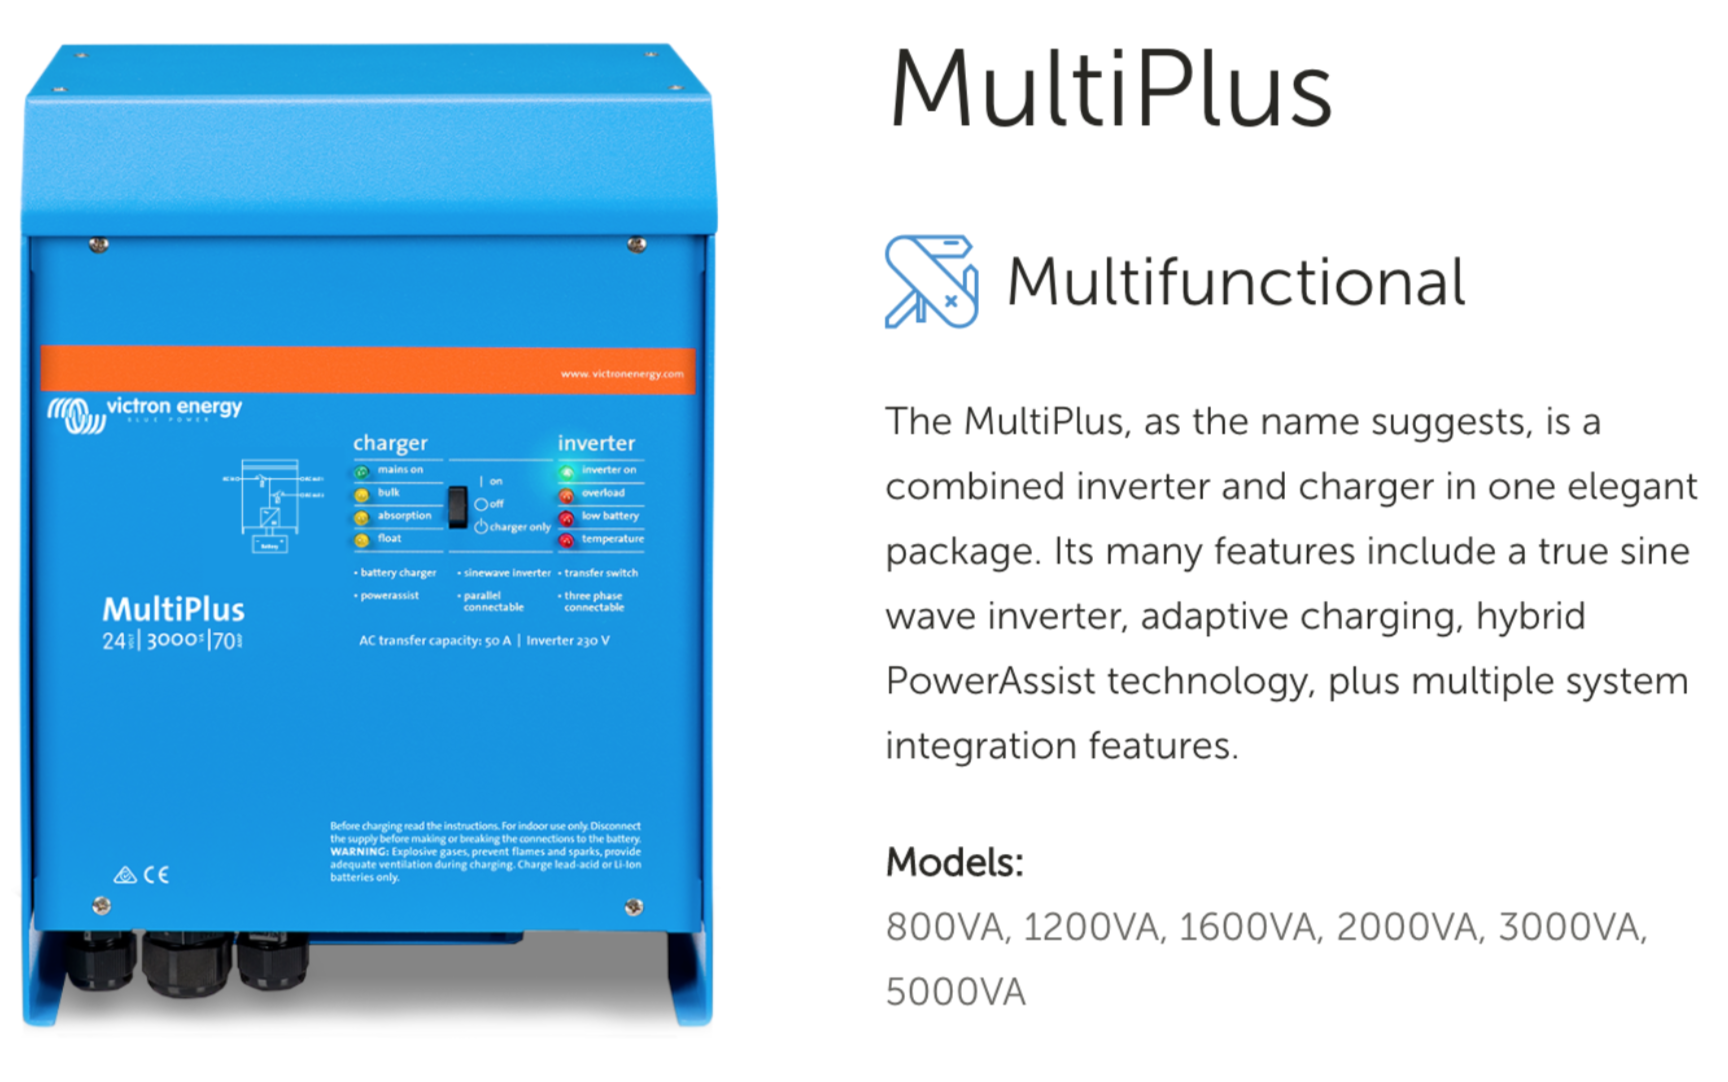
\includegraphics[width=\textwidth]{images/victron_multiplus.png}\\
  
  \end{column}
  \begin{column}{0.45\textwidth}
    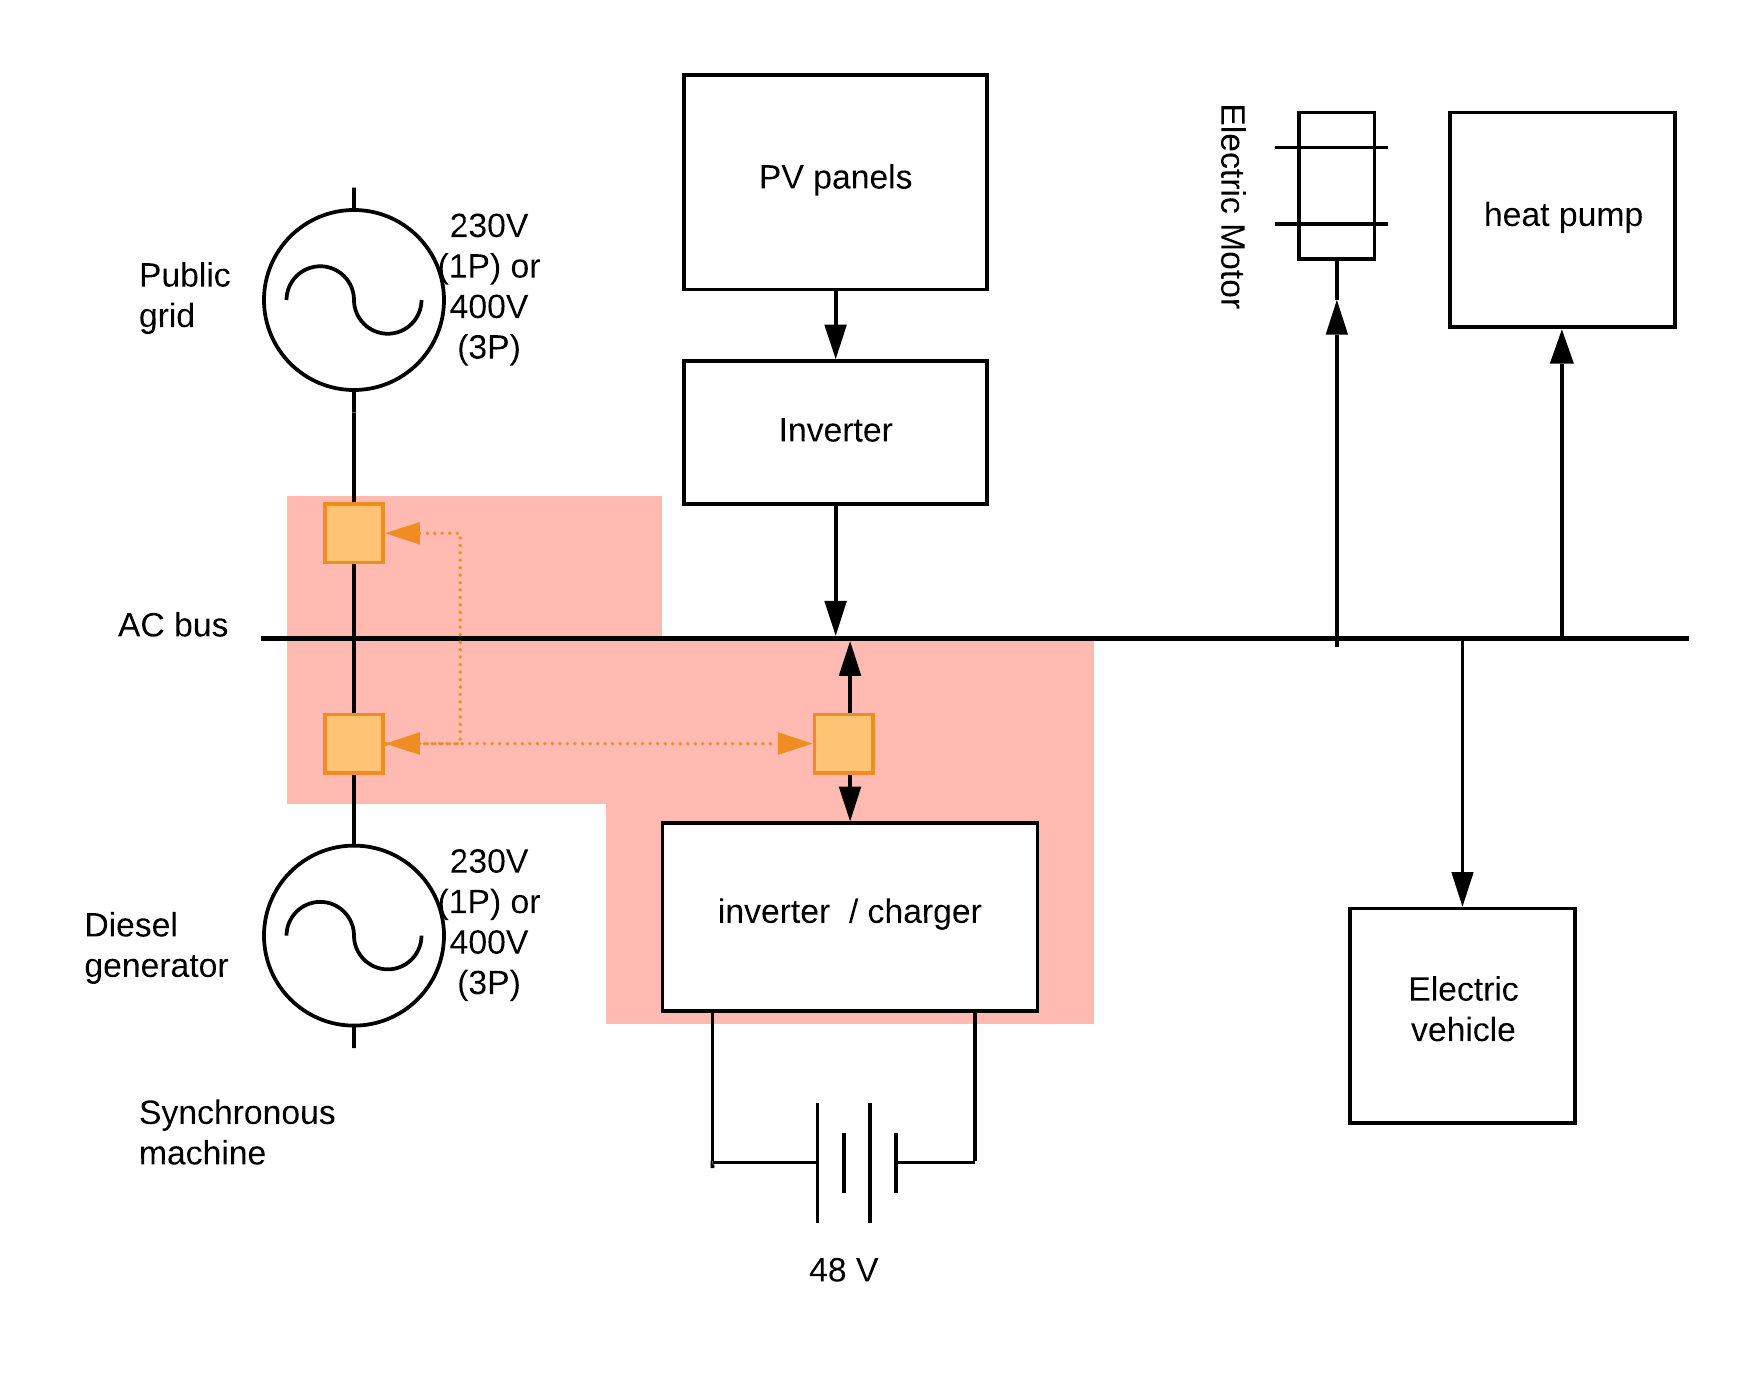
\includegraphics[width=\textwidth]{images/AC_coupling_PCC.png}
  \end{column}
\end{columns}
Source: website of Victron.

\end{frame}

\begin{frame}[allowframebreaks]{Characterizing power distribution architectures based on how power conversion is performed}
\begin{itemize}
  \item Centralized: power conversion is performed at a single power electronic interface.
\begin{columns}
  \begin{column}{0.45\textwidth}
    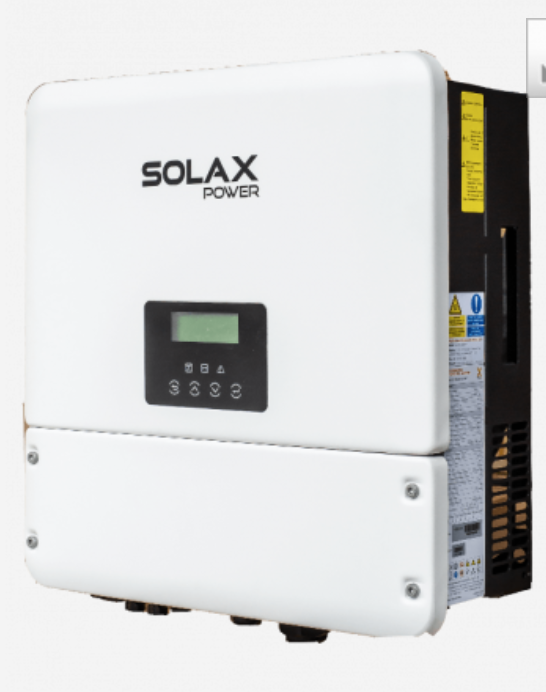
\includegraphics[width=0.6\textwidth]{images/solax.png}\\
  
  \end{column}
  \begin{column}{0.45\textwidth}
    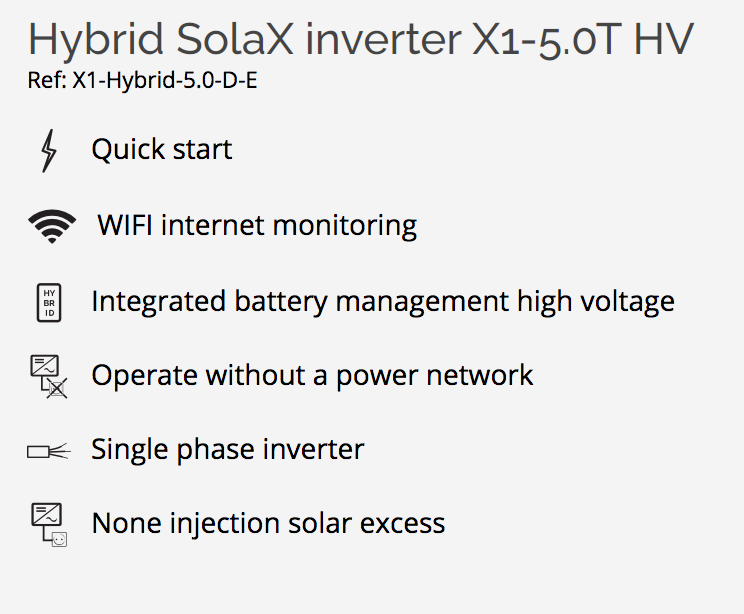
\includegraphics[width=0.9\textwidth]{images/solax_descr.png}
  \end{column}
\end{columns}
\item Distributed: power conversion functions are spread among converters
\begin{itemize}
  \item may lead to parallel or cascade structures
\end{itemize}
\end{itemize}
\end{frame}


\section{DC microgrids}

\begin{frame}{DC microgrids}
\begin{itemize}
  \item The distribution system is DC
  \item Requires DC to DC converters to adapt voltage to devices
  \item DC to AC to power AC loads, or to inject in the public grid
  \item AC to DC to convert AC generation to DC (e.g. from public grid to microgrid)
  \item DC microgrids are not widespread but gain some interest
\end{itemize}
\end{frame}

\begin{frame}{DC microgrids example}
\begin{center}
  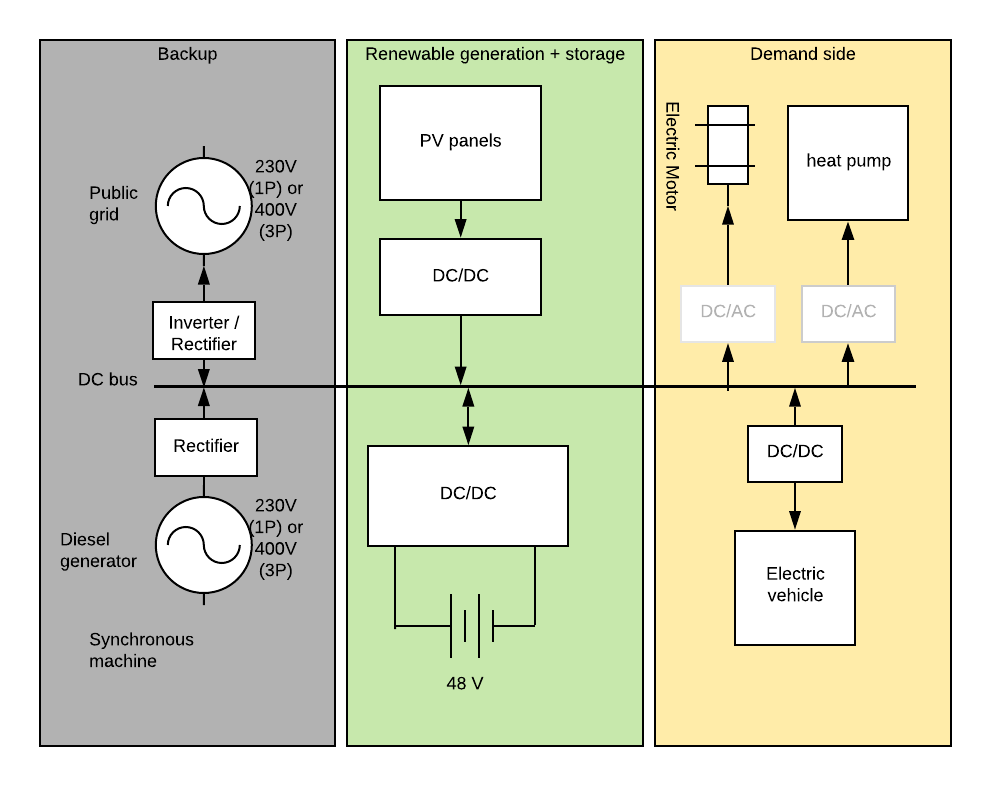
\includegraphics[width=0.6\textwidth]{images/DC_coupling.png}
\end{center}

\end{frame}

\begin{frame}{DC vs AC: pros}

  \begin{columns}
  \begin{column}{0.45\textwidth}
  \begin{itemize}
  \item DC systems enable a simpler integration of DERs, since many of them are either DC by nature or require a DC interface anyway
  \item Parallel distributed architectures are simpler to realize in DC: unnecessary frequency control and phase synchronization
  \item Frequency control is not necessary in DC systems, unwanted harmonic content may by easier to filter too
  \end{itemize}
  \end{column}
  \begin{column}{0.45\textwidth}
    \begin{itemize}
      \item Autonomous distributed control harder in DC than in AC because no information carried through the signal (frequency, phase)
      \item There are stability issues due to DCDC conversion stages
      \item It is more difficult to clear fault currents: the signal "does not go through zero". Hence protections are more costly and harder to set up.
    \end{itemize}
  \end{column}
\end{columns}
\end{frame}

\section{Rules for connecting DER to the grid}

\begin{frame}[allowframebreaks]{Synergrid}
\textbf{Synergrid} is the federation of electricity and gas network operators in Belgium. 
Synergrid establishes prescriptions for a series of topics related to distribution systems.

In the "Technical Prescription C10/11 of Synergrid, edition 2.1 (01.09.2019) (English translation)", you can find the rules that apply to a new installation.\\
\vspace{1cm}
"This document C10/11 lays down the technical requirements relating to the connection of power generating plants capable to operate in parallel to the distribution network.
The objectives of this document are the following:
\begin{itemize}
  \item ensure proper operation of the distribution networks;
  \item improve the safety of staff active in these networks;
  \item protect the distribution network's infrastructure;
  \item and contribut to the general system stability. "
\end{itemize}

\end{frame}\begin{frame}{Application domain of C10/11}
Applies to:

\begin{itemize}
  \item Plants $<25 \mathrm{MW}$ connected to the distribution grid
  \item Any energy source
  \item Without limitation regarding the possibility of actually injecting energy to the distribution network; this means, for example, that it is also applicable to power-generating plants equipped with a zero export relay. (...)
  \item ...
\end{itemize}

But not to:

\begin{itemize}
  \item Off-grid systems
  \item Backup systems (not actually able to feed in the grid)
  \item ... (elevators)
\end{itemize}

\end{frame}

\begin{frame}{Special cases}
A power backup system (as specified in § 4.1.9) will only operate in parallel with the distribution network for a short time in the following sporadic cases:

\begin{itemize}
  \item During tests
  \item In case of islanding / reconnection after a network faults ("make-beforebreak")
  \item ...
\end{itemize}

There are maximum durations depending on the cases.\\

\end{frame}


\begin{frame}[allowframebreaks]{Maximum power limits for a small power-generating plant}
\begin{center}
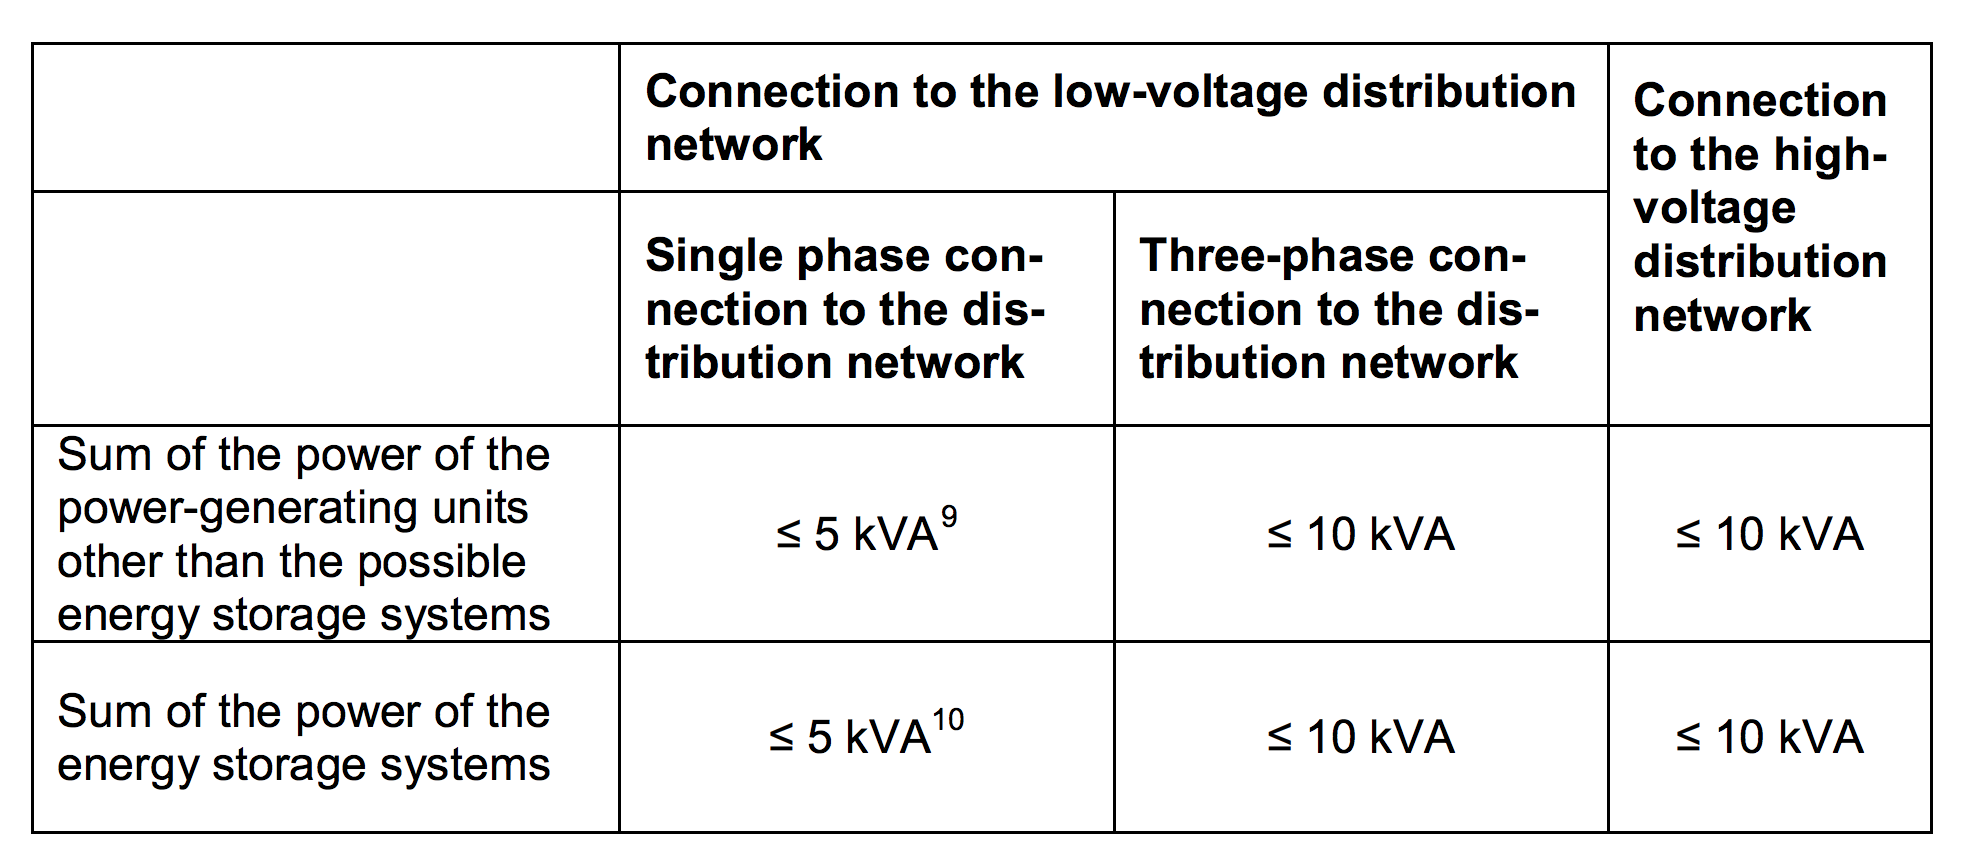
\includegraphics[width=0.7\textwidth]{images/max_power_limits_C10.png}
\end{center}

\begin{itemize}
  \item Each power-generating unit must be equipped with an \textbf{automatic separation system}
  \item If the power-generating plant includes an energy storage system,
  \begin{itemize}
    \item an EnFluRi sensor must be provided to control the power injected on the distribution network.
    \item the EnFluRi sensor is a directional power sensor having a communication link with the energy storage system.
    \item the power injected into the distribution network is limited to the maximum power of the other means of power-generation.    
  \end{itemize}
\end{itemize}

\end{frame}

\begin{frame}{Settings of the automatic separation system (Annex C)}
\begin{center}
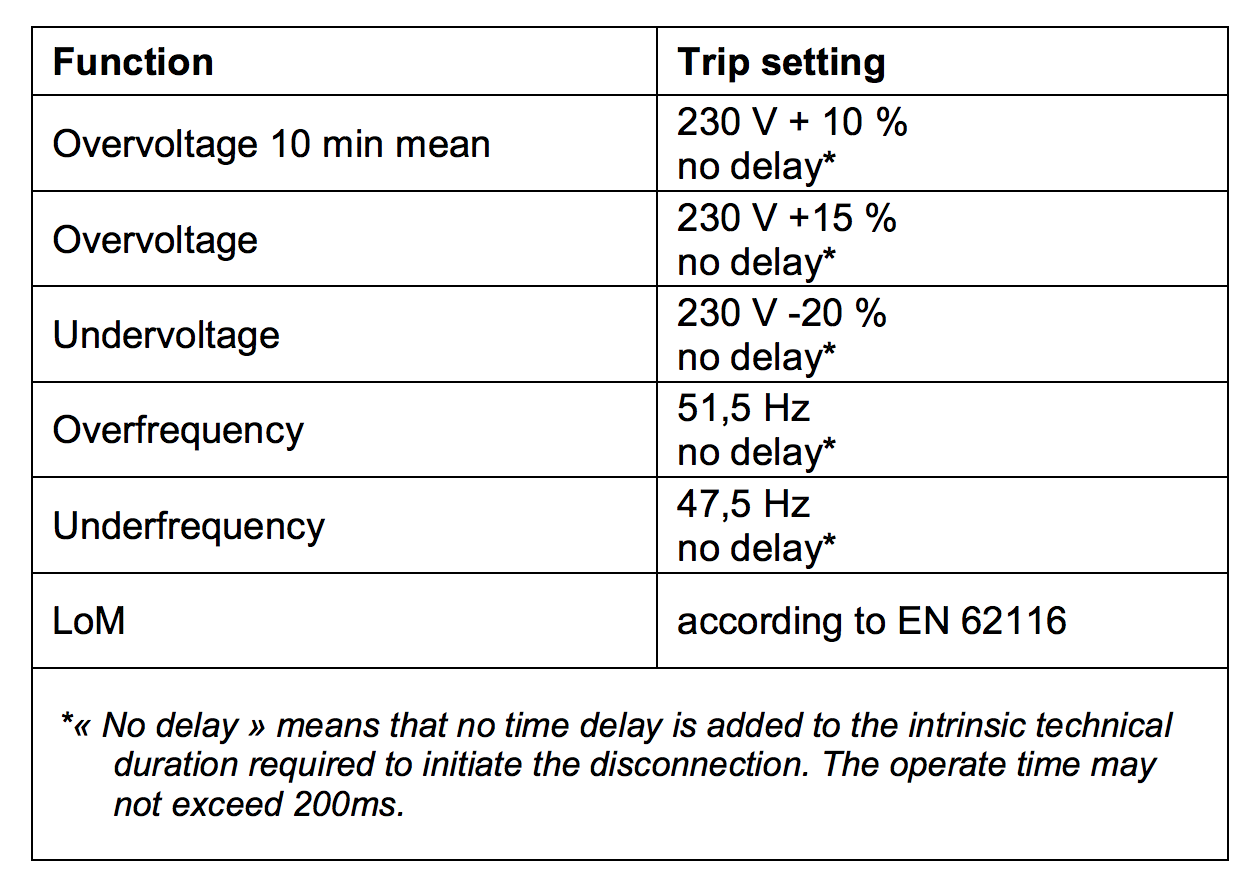
\includegraphics[width=0.6\textwidth]{images/settings_ASS.png}
\end{center}
\end{frame}

\begin{frame}{Syncrocheck}
The power-generating units which synchronize with the voltage on the distribution network (such as synchronous machines, island equipment ...), have to be equipped with a synchrocheck relay (equipped with a synchroscope) of a type homologated by Synergrid.

The synchrocheck is set as follows unless determined otherwise by the DSO:

\begin{itemize}
  \item Voltage difference < $5 \%$
  \item Phase difference $<5^{\circ}$
  \item Observation time $=0,5$ seconds
\end{itemize}

\end{frame}

\begin{frame}{Technical basic requirements regarding the power generating units (Annex D)}
E.g. Specific for a small power-generating plant (D.7.1.1)

By default, the power generation unit must operate according to the following rules:

\begin{itemize}
  \item When the voltage $\leq 105 \% U_{n}: \cos \phi=1(Q=0)$
  \item When the voltage $>105 \% U_{n}$ : free operation with $1 \geq \cos \phi>0.9$ underexcited. (no overexcited operation allowed)
\end{itemize}
\end{frame}




\section{A first microgrid demonstration Lab visit}

\begin{frame}{Assignment}
By teams of 2, write a little report and draw an electrical diagram of the demonstration board:

\begin{itemize}
  \item wiring diagram
  \item protections
  \item equipment ratings (voltage, current, power)
  \item types of controllers and regulations
  \item cable sections
  \item try to get some datasheets to understand how components work, can do and cannot do
\end{itemize}
\end{frame}

